%!TEX encoding = UTF-8 Unicode
% Template kindly provided by Lucy Strang (2021), as a modified version of Dissertate, 
% with Unimelb style changes
\documentclass[School=Unimelb]{Dissertate}

%-------- Custom additions
% Line number mode - useful during writing/reviewing
\usepackage[left]{lineno}
% For subfigures
\usepackage{subcaption}
% For appendices in a chapter
\usepackage{appendix}
% Honestly I don't remember what this does but I'm too scared to remove it
\usepackage{chngcntr}
% Allows multiple rows/columns in tables
\usepackage{multirow}
% For template demo
\usepackage{lipsum}


% Table of contents depth
\setcounter{tocdepth}{2}

%-------- Process flows & tikz


\usepackage{tikz}
\usetikzlibrary{shapes, arrows, positioning}



%-------- Multicol in bib
\usepackage{multicol}
\setlength{\columnsep}{1cm}
\renewcommand{\bibpreamble}{\begin{multicols}{2}}
\renewcommand{\bibpostamble}{\end{multicols}}


%-------------COMMANDS - SHORTCUTS --------%

% put your shortcuts here

%-------------COMMANDS - UNITS --------%

\newcommand{\hr}{\, {\rm hr}}
\newcommand{\kyr}{\, {\rm kyr}}
\newcommand{\hz}{\, {\rm Hz}}
\newcommand{\tesla}{\, {\rm T}}


%-------------COMMANDS - EDITING --------%
\newcommand{\todo}[1]{{\color{red}~\textsf{[{\bf TODO}: #1]}}} %todos

%-------------COMMANDS - BIB --------%

% shortcuts used by NASA/ADS
\newcommand\aj{The Astronomical Journal}
\newcommand\apj{The Astrophysical Journal}
\newcommand\apjl{The Astrophysical Journal Letters}
\newcommand\apjs{The Astrophysical Journal Supplement Series}
\newcommand\mnras{Monthly Notices of the Royal Astronomical Society}

% Formats bibliography spacing
\newlength{\bibitemsep}\setlength{\bibitemsep}{.2\baselineskip plus .05\baselineskip minus .05\baselineskip}
\newlength{\bibparskip}\setlength{\bibparskip}{0pt}
\let\oldthebibliography\thebibliography
\renewcommand\thebibliography[1]{%
  \oldthebibliography{#1}%
  \setlength{\parskip}{\bibitemsep}%
  \setlength{\itemsep}{\bibparskip}%
}


\author{Julian Brian Carlin}
\begin{document}
\graphicspath{{./figures/}}
% the front matter
\frontmatter

\linenumbers


% include each chapter...
%\setcounter{chapter}{-1}  % start chapter numbering at 0
\chapter{A long-expected party}
\label{chap:chap1}

An arbitrary reference to an astrophysics paper to demonstrate referencing. \citep{AasiAbadie2013}

\lipsum[1-2]

\section{A section}
\lipsum[5]
\begin{itemize}
\item Example of a list
\item It has two entries
\end{itemize}
\subsection{A subsection}
\lipsum[4]

\begin{figure}[h]
  \centering
  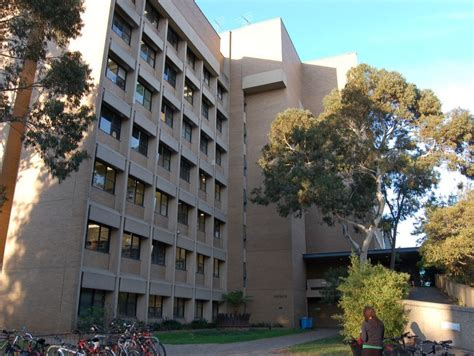
\includegraphics[width=0.9\linewidth]{figures/davidcaro.png}
  \caption{\label{fig:davidcaro} The asbestos tower of academia.}
\end{figure}

\lipsum[5-10]



 
\singlespacing

% the back matter
\clearpage
\phantomsection
% Change bib name to references
\addcontentsline{toc}{chapter}{References}
% Stylefile - swap as needed
\bibliographystyle{mnras}
% Make reference font very small
{\scriptsize
  \bibliography{thesis}{}}



\end{document}